\documentclass[a4paper,11pt]{scrartcl}
%\documentclass[a4paper,11pt]{article}
%\documentclass{article}
%\usepackage{ams}


\usepackage{fancyhdr, blindtext}
\usepackage{hyperref}
\usepackage{url}
\usepackage{graphicx}
%\usepackage{booktabs}
\usepackage{tabularx}
\usepackage{todo}
\usepackage{longtable}
\usepackage[utf8]{inputenc}
\usepackage{latexsym}
\usepackage{eurosym}
\usepackage{xspace} 
\usepackage{algorithmic}
\usepackage{algorithm}
\usepackage{listings}
\usepackage{verbatim}
\usepackage{tikz}
\usetikzlibrary{shapes,arrows,fit,calc,positioning,automata}

\usepackage{colortbl}
\usepackage{ulem}
\usepackage{verbatim}
\usepackage{multirow}
\usepackage{colortbl}
\usetikzlibrary{arrows,snakes}
\usepackage[margin=2.0cm,tmargin=2.5cm,bmargin=3.5cm]{geometry}

\newcommand{\changefont}[3]{
\fontfamily{#1} \fontseries{#2} \fontshape{#3} \selectfont}
 \renewcommand{\familydefault}{\sfdefault}

\newcommand{\authEnc}{Authenticated Encryption\xspace}
\newcommand{\bacpa}{BACPA\xspace}

\newcommand{\stateUninit}{\textsc{uninitialized}\xspace}
\newcommand{\stateInit}{\textsc{initialized}\xspace}
\newcommand{\stateCreated}{\textsc{constructed}\xspace}
\newcommand{\stateDestroyed}{\textsc{destroyed}\xspace}
%\input{../../phd/thesis/newcmds.tex}
\newcommand{\paper}[1]{#1}

\definecolor{csblue}{rgb}{0.32,0.47,0.85}
\definecolor{csbluelightformer}{rgb}{0.37,0.47,0.74}
\definecolor{csbluelight}{rgb}{0.41,0.52,0.81}
\definecolor{csorange}{rgb}{0.95,0.56,0.25}
\fancyhead{}
%\fancyfoot{}

\fancyheadoffset[L]{0.9cm}
\fancyheadoffset[R]{0.4cm}
\renewcommand{\headrule}{\hbox to\headwidth{%
  \color{csbluelight}\leaders\hrule height \headrulewidth\hfill}}

\renewcommand{\headrulewidth}{1.2pt}
\fancyhead[R]{\hspace{-1.9cm}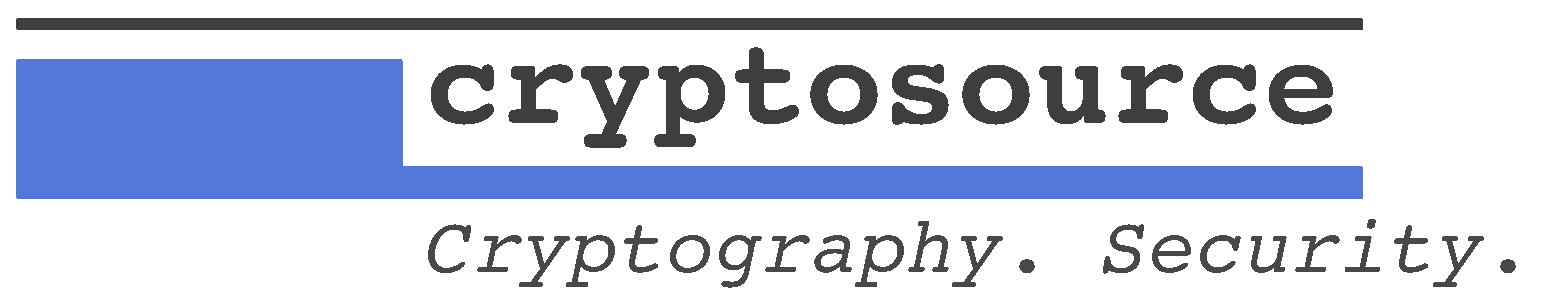
\includegraphics[width=6cm]{cs_logo.eps}}
\fancyhead[L]{flea cryptographic library 
\thisFleaVersion\\manual}
\fancyfoot[C]{\vspace{-0.3cm}\thepage}
\pagestyle{fancy}

%\ULWallPaper{bg.jpg}
\usepackage{eso-pic}
\newcommand\BackgroundIm{
  \put(5,-21){
    \parbox[b][\paperheight]{\paperwidth}{%
      \vfill
        \centering
        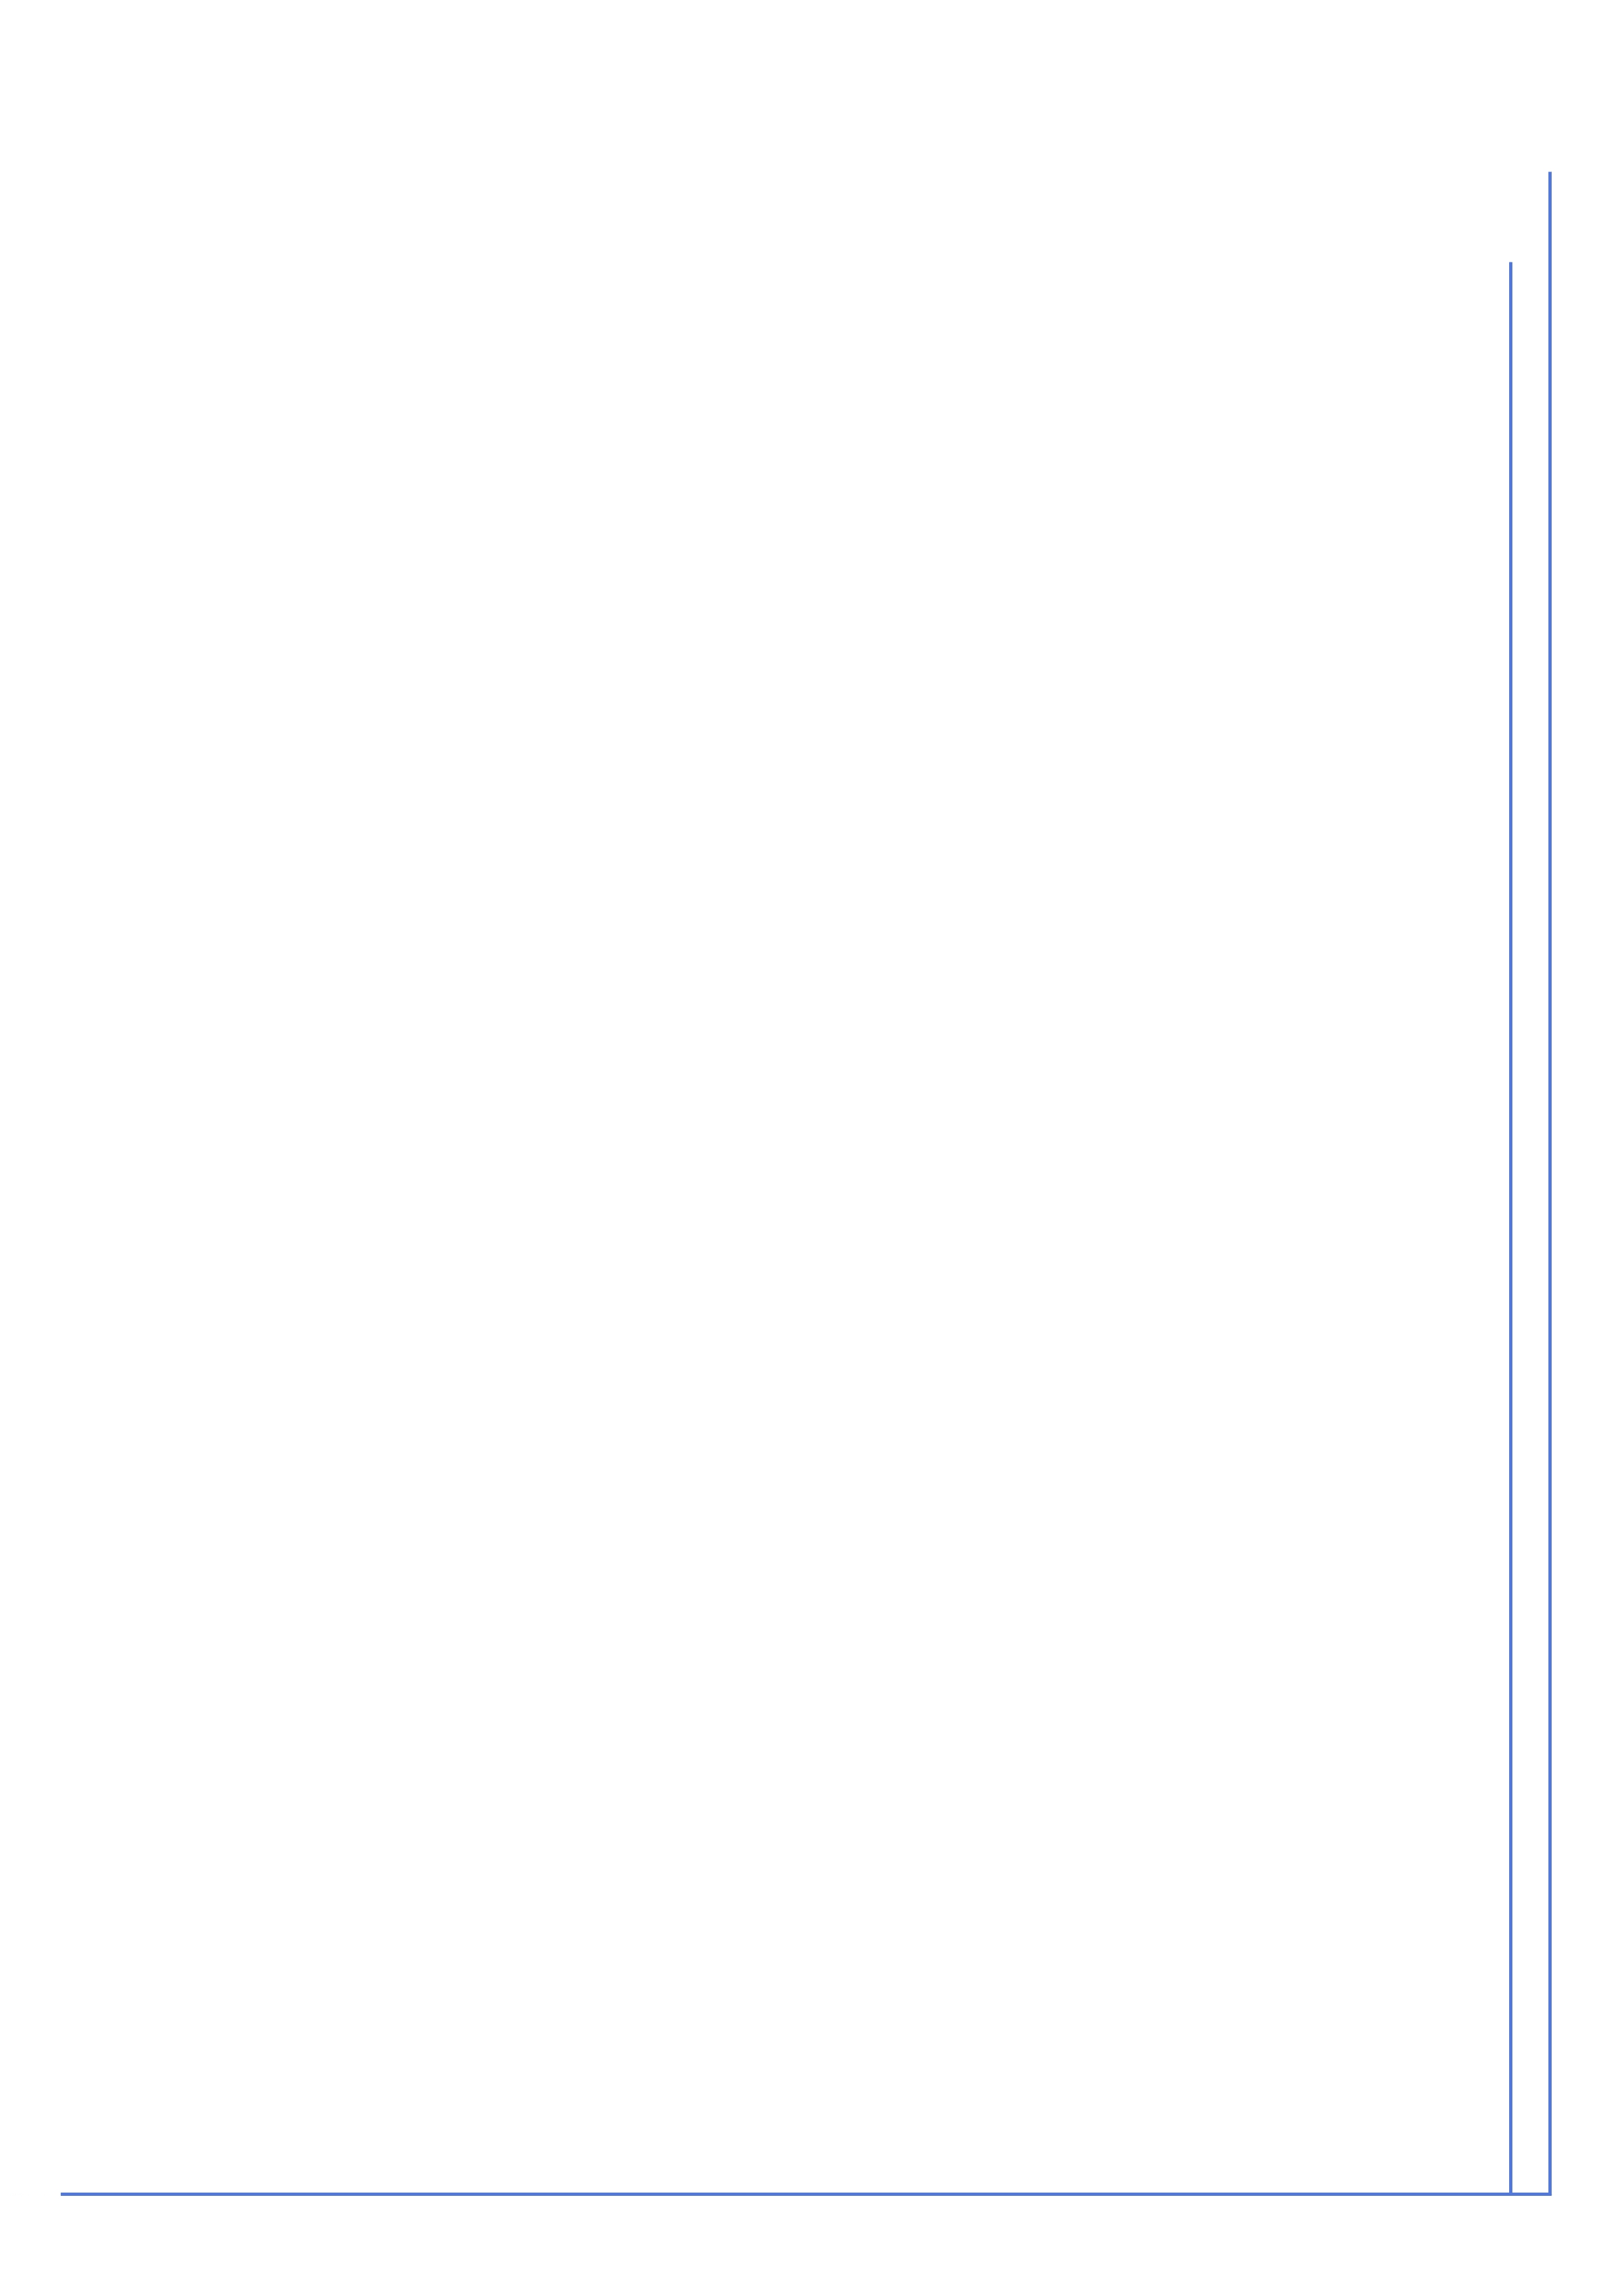
\includegraphics[height=\paperheight,width=\paperwidth,
        keepaspectratio]{bg.jpg}%
          \vfill
    }}}

        \renewcommand*\contentsname{\newline Contents}
\begin{document}
\AddToShipoutPicture{\BackgroundIm}
\changefont{cmss}{m}{n}
%\tikzset{XOR/.style={draw,circle,append after command={
%        [shorten >=\pgflinewidth, shorten <=\pgflinewidth,]
%        (\tikzlastnode.north) edge (\tikzlastnode.south)
%        (\tikzlastnode.east) edge (\tikzlastnode.west)
%        }
%    }
%}



\lstset{language=C,
  emph={int,char,double,float,unsigned,flea_u8_t,flea_al_u8_t,flea_u16_t,flea_al_u16_t,flea_u32_t,
  flea_bool_t, flea_mutex_func_set_t}, emphstyle={\color{csblue}},
frame=none,basicstyle=\ttfamily\scriptsize,columns=flexible,xleftmargin=0.9cm,float=htb,captionpos=b,breaklines=true }

\newcommand{\code}[1]{\texttt{\detokenize{#1}}}
\newcommand{\serverCtx}{\code{flea_tls_server_ctx_t}}
%\newcommand{\serverCtx}{\texttt{flea}}
\newcommand{\clientCtx}{\code{flea_tls_client_ctx_t}}
\newcommand{\funcLibInit}{\code{THR_flea_lib\-__init()}\xspace}
\newcommand{\funcSaveRngState}{\code{flea_\-prng_\-save_f}\xspace}

\newcommand{\thisFleaVersion}{v1.2\xspace }

\DeclareRobustCommand{\eg}{e.g.\@\xspace}
\DeclareRobustCommand{\ie}{i.e.\@\xspace}
%\mainmatter              % start of the contributions
%
\title{flea cryptographic library \thisFleaVersion\\{\LARGE manual} }

\author{cryptosource GmbH,
  Darmstadt\\\url{flea@cryptosource.de}\\\url{www.cryptosource.de}\vspace{0.5cm}\\
\includegraphics[width=7cm]{logo.png}}

\maketitle              % typeset the title of the contribution

%\begin{abstract}
%\end{abstract}

\newpage

\setcounter{tocdepth}{3}
\vspace{1cm}
\tableofcontents

\newpage

\section{Introduction}
flea, the acronym of ``flexible lightweight efficient algorithms'' is a
cryptographic library written in C and intended for resource
constrained devices. 
%In the current version it
%comes with a basic set of the most fundamental symmetric and asymmetric
%algorithms. 
It is especially intended to run on bare microcontrollers without
any operating system support. However, it can be readily run on standard PCs as
well. The current release of flea only supports 32-bit architectures but
compiles and runs also on 64-bit machines.


 
  \section{The fleaTLS API}
  An API documentation is available at \todo{TODO:URL}. 

  In the function parameter lists, \verb#[in]#, \verb#[out]#, and
  \verb#[in/out]# specifies whether a parameter is a mere input, a mere output,
  or both for the function. Here, a parameter is considered as an output if it
  it is a pointer and the object it points to is potentially updated by the
  function. An output parameter is guaranteed to be updated by the function to
  the value specified in the API documentation if the function returns without
  indicating an error, i.e. when it returns \code{FLEA_ERR_FINE}.

  A function parameter ending \code{_mbn} stands for ``may be null'' and
  indicates that the caller my supply a null pointer for the parameter.
\section{Getting started with flea}

  In order to get easily started with flea, the library is shipped with a CMake
  configuration to build it on standard Linux. In the
  flea directory, the command sequence 
  \begin{verbatim}
  cmake .
  make -j4
  ./build/unit_test
  \end{verbatim}
  can be issued to build the library, the unit tests, and execute the tests.

  However, the library is shipped in a state in which it produces two
  compilation errors. This is due to the fact that for the secure operation of
  the random number generator (RNG) of the library the user has to implement two
  functions for the persistence of the RNG state. The source code contains
  guidance how to quickly repair these compilation errors with a workaround,
  which, however, leads to an insecure build of the library that must not be
  used in production code. In Section \ref{secRng} we give guidance on how to use
  the RNG safely.

  \section{Compile-Time Configuration}

The library offers various compile-time
configuration options, such as 
\begin{itemize}
  \item the set of algorithms to include in the library
  \item use of stack memory only or the additional use of heap memory,
  \item configuration of the maximal key sizes for the determination of the
    buffer sizes in stack-only mode,
  \item buffer overwrite detection through canary values at the start and end of
    each buffer,
  \item various trade-offs concerning code-size, RAM demand and speed.
  \end{itemize}

  The compile-time configuration of the library is completely managed by a
  preprocessor framework. All configuration options can be set in the file
  \verb#build_cfg/general/build_config.h#, making it easy to configure the
  library on embedded platforms without any dependency on the build system.

  In order to build the library on an arbitrary 32-bit platform, the following
  directories must be in the compiler's include path:
  \begin{itemize}
    \item \verb#include#
    \item \verb#include/api#
    \item \verb#test/include# (in case that the unit tests shall be build)
    \item \verb#build_cfg/pltf_spec/32bit_default#
    \item \verb#build_cfg/general#
  \end{itemize}

\section{Random Number Generation }
\label{secRng}

As random number generation is a precondition for many cryptographic operations,
fleaTLS features support for random number generation. On the one hand, there
are there is the type \code{flea_ctr_mode_prng_t}, defined in the file
\code{ctr_mode_prng.h}, for the instantiation of
pseudo random number generator (PRNG) objects, on the other hand there is the flea's
global random number generator (RNG). Its interface is defined in the file
\code{flea/rng.h}. flea's global RNG is based on a
\code{flea_ctr_mode_prng_t}, but features additional functions and has a
specific life cycle.

\begin{figure}

\tikzstyle{funcBlock} = [
rectangle, rounded corners=2pt, minimum width=4.2cm,
    minimum height=1cm, color=white, draw=darkgray, fill=csblue, node distance
= 1.1cm]

\tikzstyle{seedBlock} = [
rectangle, rounded corners=9pt, minimum width=2cm,
    minimum height=1cm, color=white, draw=darkgray, fill=orange, node distance
= 2.5cm]
\tikzstyle{stateBlock} = [
rectangle, rounded corners=2pt, minimum width=2cm,
    minimum height=1cm, color=white, draw=darkgray, fill=blue, node distance
= 2.1cm]

\tikzstyle{poolBlock} = [
rectangle, rounded corners=2pt, minimum width=2cm,
    minimum height=0.5cm, color=white, draw=darkgray, fill=lightgray, node distance
= 0.4cm]
\tikzstyle{codeBlock} = [
node distance = 1.1cm, align = left]

\tikzset{
      myarrow/.style={->, >=latex', shorten >=3pt, thick},
      myDashedArrow/.style={->, >=latex', shorten >=1pt, dashed, thick},
      myarrowRev/.style={-<, >=latex', shorten >=1pt, thick},
      myline/.style={ >=latex', shorten >=1pt, thick},
      mylabel/.style={text width=7em, text centered}
    }
\begin{tikzpicture}

\node[stateBlock] at (0,0) (stateZero) {state};
\node[funcBlock, right = of stateZero] (funcZero) {\funcLibInit};
\node[right = of funcZero] (argsZero) {seed [,\funcSaveRngState]};
\node[seedBlock, left = of stateZero.west] (seedFile) {seed file};
\node[poolBlock, above = of stateZero.north] (poolZero) {pool};
\draw[myarrow] (argsZero) -- (funcZero);
\draw[myarrow] (funcZero) -- (stateZero);
\draw[myarrow] (stateZero.west) -- node[midway, above, align=left]
{\code{flea\_prng\_}\\\code{save\_f}} (seedFile.east);
\draw[myarrow] (seedFile.north) -- node {} ++(0, 2cm) -| node [midway,above]
{after initial power cycle} ($(argsZero.north
west)+(0.5,0)$);
%\draw[->, thick] ($(initHs.west) - (1,0)$) -- ($(close.west) - (1,0)$);

\node[stateBlock, below = of stateZero, node distance = 4cm] (stateOne) {state};
\node[funcBlock, right = of stateOne, align=left] (funcOne) {\code{THR\_flea\_rng}\\\code{\_\_randomize()}};
\node[right = of funcOne] (argsOne) {output};
\node[poolBlock, above = of stateOne.north] (poolOne) {pool};
\draw[myarrow] (funcOne) -- (argsOne);
\draw[myarrow] (stateOne) -- (funcOne);


\node[stateBlock, below = of stateOne, node distance = 4cm] (stateTwo) {state};
\node[funcBlock, right = of stateTwo,align=left] (funcTwo)
{\code{THR\_flea\_rng\_\_re}\\\code{seed\_volatile()}};
\node[right = of funcTwo] (argsTwo) {seed data};
\node[poolBlock, above = of stateTwo.north] (poolTwo) {pool};
\draw[myarrow] (argsTwo) -- (funcTwo);
\draw[myarrow] (funcTwo) -- (stateTwo);


\node[stateBlock, below = of stateTwo, node distance = 4cm] (stateThree) {state};
\node[funcBlock, right = of stateThree,align=left] (funcThree)
{\code{THR\_flea\_rng\_\_re}\\\code{seed\_persistent()}};
\node[right = of funcThree] (argsThree) {seed data};
\node[poolBlock, above = of stateThree.north] (poolThree) {pool};
\draw[myarrow] (stateThree.west) -| node[midway, above, align=left] {\code{flea\_prng\_}\\\code{save\_f}} (seedFile.south);
\draw[myarrow] (argsThree) -- (funcThree);
\draw[myarrow] (funcThree) -- (stateThree);


\node[stateBlock, below = of stateThree, node distance = 4cm] (stateFour) {state};
\node[funcBlock, right = of stateFour, align=left] (funcFour)
{\code{flea\_rng\_\_feed}\\\code{\_low\_entropy\_}\\\code{data\_to\_pool()}};
\node[right = of funcFour] (argsFour) {seed data};
\node[poolBlock, above = of stateFour.north] (poolFour) {pool};
\draw[myarrow] (argsFour) -- (funcFour);
\draw[myarrow] (funcFour.west) -- node {} ++(-0.5cm,0) |- (poolFour.east);

\node[below = of funcFour] (dotsFeed) {\Huge \ldots};
\node[node distance=2.9cm, left = of dotsFeed ] {\Huge \ldots};


\node[stateBlock, node distance = 3cm, below = of stateFour] (stateFive) {state};
\node[funcBlock, right = of stateFive,align=left] (funcFive) {\code{THR\_flea\_rng}\\\code{\_\_randomize()}};
\node[right = of funcFive] (argsFive) {output};
\node[poolBlock, above = of stateFive.north] (poolFive) {pool};
\node[node distance = 0.7cm, left = of poolFive, align = left] (poolTextFive)
{reseed the state\\with the pooled\\ entropy after \\threshold is \\reached};
\draw[myarrow] (funcFive) -- (argsFive);
\draw[myarrow] (stateFive) -- (funcFive);
\draw[myarrow] (poolFive) -- (stateFive);

\draw[->,dashed] ($(funcZero.north east)+(0.5,0.5)$) -- ($(funcFive.south east) + (0.5,-1.5)$);
\end{tikzpicture}

\label{figRngLifeCycle}
\caption{Overview of the life cycle of fleaTLS' global RNG. The dashed line represents
fleaTLS' API and shows the direction of time. 
The functions after \funcLibInit may actually be called in an arbitrary order.
The sequence shown here serves merely as an example.
The paths labelled
with \funcSaveRngState are only actually relevant if the corresponding function
pointer is provided to the function \funcLibInit. Refer to the text for a
detailed explanation.}
\end{figure}

\subsection{fleaTLS' Global RNG's Life Cycle}
\label{secRngLifeCycle}
The global RNG's life cycle starts with the call to the function
\code{THR_flea_lib\-__init()}. This function takes an initial seed value for
the global RNG as its argument. It the caller's responsibility to provide a high
entropy seed of an appropriate length here. fleaTLS makes no checks in this
respect. 

The function \funcLibInit also supports the configuration of the seed file
management support of fleaTLS. For details seed Section \ref{secSeedFile}.


After the initialization of the global RNG through the call to
\code{THR_flea_lib\-__init()}, it can be used for the generation of random
byte arrays by the function \code{THR_flea_rng__randomize()}. Furthermore,
it is possible to reseed the generator using one of the functions
\code{THR_flea_rng__reseed_volatile()} or 
\code{THR_flea_rng__reseed_persistent()}. The former updates the global
RNG's internal state with the provided seed data. The latter does the same, but
also updates the managed seed file (see Section \ref{secSeedFile}).

\subsection{Reseeding the Global RNG with Low Entropy Data}
\label{secLowEntropyReseed}
fleaTLS' global RNG also features a function for the feeding of low entropy seed
data in the form of 32-bit values, namely
\code{flea_rng__feed_low_entropy_data_to_pool()}. This function is
intended to received for instance time stamp counter values from asynchronously
triggered events in order to provide fresh entropy to the global RNG. The caller
is required to provide an estimate of the entropy contained in that value in
bits. This estimation is used for the management of fleaTLS' global RNG's
entropy pool. In this pool the low entropy feeds are accumulated. Whenever the
accumulated estimated entropy reaches the threshold of 128 bits, in the next
call to the function \code{THR_flea_rng__randomize()} the global RNG will
reseed itself with the content of the entropy pool. 

The function \code{flea_rng__feed_low_entropy_data_to_pool()} does not
use any mutexes to prevent concurrent access. This is intentional, since it is
expected to be called from interrupt routines which may never be blocked.
fleaTLS' functions which access the
entropy pool are written in such a way that a potentially concurrent access does
not cause program errors. In actual cases of concurrent accesses, it may happen that
the fed low level entropy is not optimally transferred to the pool or that a
randomize function prematurely uses the pool for reseeding the RNG state. Any
such event does not actually degrade security of the RNG state, but only reduces the effect of
the pooled entropy under certain conditions to a certain degree. If an
implementer considers the pooling functionality essential to the secure
operation of his product, and actually expects simultaneous calls to the functions
\code{flea_rng__feed_low_entropy_data_to_pool()} and
\code{THR_flea_rng__randomize()} with a high frequency, a mutex mechanism should be implemented.

\subsection{Seed Management}
\label{secSeedFile}
The default recommended approach is to make use of fleaTLS' support for
the management of a continously managed seed file. In this case, the caller
of \funcLibInit should provide the optional parameter for a function of type
\code{flea_prng_save_f} to \funcLibInit. This function has to be implemented
by the user of fleaTLS. It will be called by
fleaTLS whenever the function \code{THR_flea_rng__reseed_volatile()} from
the global RNG's interface is called. In this case the global RNG produces a new
random output which is provided to the \code{flea_prng_save_f} as the
argument. The function is expected to save the byte array it received in its
argument to non-volatile memory and signal any potentially occurring errors by
returning appropriate non-zero error values. The size of the byte array provided
to \funcSaveRngState is always 32 bytes.

If a \funcSaveRngState function is provided to \funcLibInit, the following seed-file-based life cycle model
is supported by fleaTLS. This model ensures secure random number generation over
all power cycles of the device under the
assumption that no malicious entity gained knowlegde of the initial seed, the
seed file managed by fleaTLS or the global RNG's state directly.

During the unique initial device initialization, \eg
during production, an initial high entropy seed is provided to the
function \funcLibInit. Furthermore, the function pointer argument of the type
\funcSaveRngState, implemented as explained above, is also provided to
\funcLibInit. In any subsequent call to \funcLibInit, the latest seed value that was
provided to \funcSaveRngState as its argument is used as the seed file argument.

The function \funcLibInit internally calls the function
\code{THR_flea_rng__reseed_persistent()}, which causes \funcSaveRngState to
invoked with freshly generated output from the global RNG. Thus during each
subsequent call to \funcLibInit, it is ensured that a fresh high entropy seed is
used to initalize the global RNG.

In order to achieve a lasting of effect of any reseedings of the global RNG
by calls to the functions  \code{THR_flea_rng__reseed_volatile()} (see
Section \ref{secRngLifeCycle} or
\code{flea_rng__feed_low_entropy_data_to_pool()} (see Section
ref{secLowEntropyReseed}), \ie a subsequent update of the seed file, client code
should occasionally call the function
\code{THR_flea_rng__reseed_persistent()}, which triggers a call to the
function \funcSaveRngState, provided that such a function was specified in the
call \funcLibInit.

\section{Using flea's API}

flea uses a macro framework to abstract object and buffer initialization as well
as error handling. This allows for greater flexibility and security for a number of reasons:
\begin{itemize}
  \item it is possible to switch between stack and heap usage for buffer allocation
  by changing a single compiler flag,
  \item the life cycles of buffers and objects are formalized and integrate
    seamless with the error handling, guaranteeing safety from resource leaks
    and errors such as use-after-free if the programming standards are adhered
    to.
\end{itemize}

From the following sections, only Sections \ref{secFleaObj} and \ref{secErrRet}
are essentially
important for users of the library since the other sections describe the
internal design of flea which is not necessary for the use of its API. But since
the test code shipped with flea, which can serve as a source of example code, is
written in the same framework, it is helpful to understand also the approaches
to error handling and buffer management outlined in the subsequent sections.
\subsection{flea's Objects}
\label{secFleaObj}
flea's objects have the following life cycle states:
\begin{itemize}
  \item \stateUninit. This state is entered by simply declaring an object on
    stack or heap without assigning any value to it. From this state, only the
    transition to the state \stateInit is allowed.
  \item \stateInit. This state is entered via one of the following means:
    \begin{itemize} 
        \item By using the macro
    \verb#FLEA_DECL_OBJ(symbol_name, object_type)# for the object declaration
    and simultaneous initialization. 
    \item Alternatively, an object in the state
    \stateUninit can make the transition to the state \stateInit by invoking the
    corresponding initialization macro.
    Their naming pattern is \verb#flea_<type>__INIT(symbol_address)#.
    In the state \stateInit, only two
    actions may be performed on the object: The object's destructor (dtor)
    function or one of its constructor (ctor) functions may be called.
\end{itemize}
  \item \stateCreated. This state can be entered in two ways
    \begin{itemize}
    \item By the calling one of the object's
    ctor functions or other functions which perform object creation. The state
    \stateCreated can only be left by calling the object's dtor function. If a
    function returns when any of its objects are in the state \stateCreated,
    then this will result in a memory leak in the case of heap mode.
    \item Alternatively, for some objects, the exist also initialization value
      macros labelled conforming to the naming pattern
      \verb#flea_<type>__CONSTR_<further specification>#. An object initialized
      with such a value is in the state \stateCreated afterwards.
  \end{itemize}
  \item \stateDestroyed. This state is entered by calling the object's dtor
    function. In this state, the dtor function may be called repeatedly (without
    any effect) or the object may be created again using a ctor function.
\end{itemize}

This is the contract offered by all class-like types of flea's API. The dtor calls should
be made even in the stack-only mode, because they wipe secret values from the
RAM before deallocation.

The flea library functions themselves realize an approach which ensures that all
requirements from flea life object cycle model are met. This approach is
described in Section \ref{fleaFuncSkel} and it is recommended to adapt it in implementations
using flea or realize a corresponding solution.


\subsection{Error Return Values}
\label{secErrRet}
Any function of flea that potentially returns an error, referred to as a throwing function, can be identified by starting with the string
\verb#THR_#. Such a function returns \verb#FLEA_ERR_FINE#, which is defined as
zero, upon success or one of the error codes define in \verb#flea/error.h# otherwise.
When calling throwing functions in flea it is necessary test their return value
and take appropriate actions if an error occured.

\subsection{Object Life Cycle and Error Handling within the flea Library Functions}
\label{fleaFuncSkel}
In order to establish a standardized and robust approach to object initialization,
object creation, object destruction and error handling, the flea library
function implementations themselves employ a dedicated macro framework. This
approach is described in the following to facilitate the understanding of the
implementation. Furthermore, it may be be adapted in the flea library user's own
code.

Specifically, any throwing function in flea is structured by the following skeleton:
\begin{verbatim}
  <declaration section>
  FLEA_THR_BEG_FUNC();
  <initialization section>
  <throwing section> 
  FLEA_THR_FIN_SEC(cleanup-code);
\end{verbatim}
In the \verb#declaration section# all variable declaration happen. Next, in the \verb#initialization section#  
all objects so far not initialized are initialized by means of the
corresponding initialization macros. Any throwing functions may only be called
after this section in the \verb#throwing section#. 
The \verb#cleanup-code# is the code that shall be executed whenever the function ends,
either by naturally running to the location of the macro call
\verb#FLEA_THR_FIN_SEC()# or because between the two macro calls an error was
thrown and not handled, causing an immediate jump to the cleanup-code. This can happen mainly due to two incidents:
\begin{itemize}
  \item An error was raised by calling the macro \verb#FLEA_THROW()#. This
    causes the routine to directly jump to the cleanup code and the function
    returns the error code raised by \verb#FLEA_THROW()#. 
  \item An error was returned by a throwing function called as
    \verb#FLEA_CCALL(THR_flea_some_function(args))#. The behaviour is the same
    as for the \verb#FLEA_THROW()# macro, i.e. a return value other than
    \verb#FLEA_ERR_FINE# causes an immediate jump to the cleanup-code. In this, the error code returned by the
    called function is returned by the current function.
\end{itemize}

It is important to stress that in order to have correct life cycle management even in the presence of errors
thrown directly in the code or returned by called functions, one essential rule must be followed:
Before any code is executed that potentially raises errors, all objects 
used within the function must have be initialized. 
  %  If only the \verb#FLEA_DECL_OBJ()# is used for the
  %  object declaration, then this is naturally achieved. 
    %If, however, any
    %objects are declared in the standard way and only initialized in the
    %initialization-section indicated above, then it is vital that no error
    %throwing code is executed in the initialization section.
%  \end{enumberate}
Following this rule ensures that the jump to the cleanup section, which
typically executes the dtors for all local objects, is possible at any time
during error-throwing code.

\subsection{Buffer Management}
The buffer management in flea is abstracted by macros in order to enable both
the abstraction from heap/stack usage and in order to enable the use of canary
values for buffer overwrite detection.

The following  macros are mainly employed for the buffer management:
\begin{itemize}
  \item \verb#FLEA_DECL_BUF(symbol_name, type, size)# declares a buffer, 
  \item \verb#FLEA_ALLOC_BUF(symbol_name, size)# allocates a buffer, 
  \item \verb#FLEA_FREE_BUF_FINAL(symbol_name)# frees a buffer,
  \item \verb#FLEA_FREE_BUF_SECRET_ARR(symbol_name, size)# also frees a buffer,
    but also overwrites the memory contents prior to that.
\end{itemize}
All buffer sizes are specified in element counts, not in bytes. However, the
user of the library, who does not intend to make use of flea's features for 
switching between stack and heap mode in his own code or use the buffer
canaries, may certainly use any explicit heap or stack buffer allocation as he
is used to.



\section{The TLS API}

flea implements the TLS 1.2 protocol for the instantiation of TLS clients and
server. 

\section{A brief description of the TLS protocol}
TLS is a protocol which allows for the establishment of secure connections
between a TLS client and a TLS server. The authenticity of the server, and
optionally that of the client is ensured by the use of X.509 certificates.
During the so-called TLS handshake the authenticity of the X.509 certificate of
the peer is verified and based on the public key presented in that certificate
a key exchange (KEX) is performed. As a result, after the TLS handshake, both
sides share a set of symmetric keys for the encryption and authentiation of the
payload data, also referred to as application data. 
At this point, both peers
can send application data to each other in a confidential and authentic manner.
The concrete cryptographic algorithms that are used during the handshake and for the
transmission of the application data, are specified by the so-called TLS
cipher suite.

\subsection{Overview of the TLS Protocol Flow}
\begin{figure}

\tikzstyle{flowBlock} = [
rectangle, rounded corners=2pt, minimum width=4cm,
    minimum height=1cm, color=white, draw=darkgray, fill=csblue, node distance
= 0.1cm]

\tikzstyle{codeBlock} = [
node distance = 1.1cm, align = left]

\begin{tikzpicture}

\node[flowBlock] at (0,0) (initHs) {Initial Handshake};
\node[right = of initHs.east] (ctor) {\code{ctor}};

\node[flowBlock, below = of initHs.south] (appData) {send/read app. data};
\node[right = of appData.east] (ad1) {\code{send\_app\_data},
\code{read\_app\_data}};

\node[flowBlock, below = of appData.south] (reneg) {renegotiation};
\node[right = of reneg.east] (ctor) {\code{renegotiate}, \code{read\_app\_data}};

\node[flowBlock, below = of reneg.south] (appData2) {send/read app. data};
\node[node distance = 0.3cm, below = of appData2.south] (any) {\Huge\ldots};

\node[flowBlock, below = of any.south] (close) {close connection};
\node[right = of close.east] (dtor) {\code{dtor}, error in any function};

\draw[->, thick] ($(initHs.west) - (1,0)$) -- ($(close.west) - (1,0)$);
\end{tikzpicture}

\caption{Overview of the potential events during the TLS protocol flow and the
associated functions of the flea TLS Client and Serve API.}
\label{figTlsSeqFlow}
\end{figure}

Figure \ref{figTlsSeqFlow} shows the potential events in the TLS protocol flow
and the associated functions of the fleaTLS client and server API. Any TLS
connections starts with a call to the ctor function of the TLS client
(\clientCtx) or server (\serverCtx) context object.

\subsubsection{Initial Handshake and Application Data Transfer}
After the initial handshake, the TLS channel is established and all subsequent
data exchanges between the peers take place over the secure TLS channel. The
main purpose of the TLS channel is the secure exchange of application data,
which is done using the fleaTLS functions 
\begin{itemize}
  \item \code{THR_flea_tls_client_ctx_t__read_app_data()}
\item \code{THR_flea_tls_client_ctx_t__send_app_data()}
\item \code{THR_flea_tls_server_ctx_t__read_app_data()}
  \item \code{THR_flea_tls_server_ctx_t__send_app_data()}
\end{itemize}

Note that in order to ensure the sending of the application over the wire a call
to 
\begin{itemize}
  \item \code{THR_flea_tls_client_ctx_t__flush_write_app_data} or
  \item \code{THR_flea_tls_server_ctx_t__flush_write_app_data}
  \end{itemize}
  is necessary since the \code{send_app_data} functions may buffer the data.

  \subsubsection{Renegotiation}
A renegotiation can be triggered either by a call to the corresponding
renegotiation function
\begin{itemize}
  \item \code{THR_flea_tls_client_ctx_t__renegotiate} or
\item \code{THR_flea_tls_server_ctx_t__renegotiate}
  \end{itemize}
  or during a call to a \code{read_app_data} function, if the peer initiates a
  renegotiation during that call which is accepted by flea.

  The conditions for accepting a renegotiation request by the  fleaTLS client or
  server are the following:
  \begin{itemize}
    \item If in the TLS client or server context object's ctor call the flag \code{flea_tls_flag_reneg__allow_insecure_reneg} is
      set, then the renegotiation request is accepted under any condition.
    \item If in the TLS client or server context object's ctor call the flag \code{flea_tls_flag_reneg__allow_only_secure_reneg} is
      set, then the renegotiation request is accepted if the peer also supports
      the Renegotiation Indication Extension and behaves correctly with respect
      to this extension.
      \item If in the TLS client or server context object's ctor call the flag \code{flea_tls_flag_reneg__no_reneg} is
      set, then the renegotiation request is declined unconditionally.
  \end{itemize}

  The closing of a connection happens when dtor function of the respective tls
  client or server context object is called. Furthermore, the connection is
  closed if an error occurs during any of the other TLS client or server context
  objects.
%TODO: FIGURE:
%handshake
%  client hello
%  server hello
%  \ldots
%tls channel
%  renegotiate
%  read/write app data

  \subsubsection{TLS Alert Handling and Sending }

  In the TLS protocol alert messages are specified as a means to signal error
  conditions to the peer. The carry a type and a level field. A variety of possible types
  is specified in the TLS standard. The level can be \emph{fatal}, indicating an error
  that mandates the ending of the connection, or \emph{warning}, indicating that,
  depending on the type of the alert, a specific action may be necessary.
  fleaTLS completely handles the treatment of incoming
  TLS alerts and sending of alerts when an error condition is met.

  If fleaTLS receives an alert the reaction is determined according to the
  following rules:
  \begin{itemize}
    \item If the alert has level \emph{fatal}, flea closes the connection and the API
        function during the execution of which the alert was received returns an
        error code.
      \item Otherwise, if the alert has level \emph{warning}, and
        \begin{itemize}
          \item if it is of type \emph{close notify}, then the connection is closed as
            well, \ie fleaTLS sends a \emph{close notify} alert to the peer itself;
          \item if it is of type \emph{no renegotiation}, and fleaTLS is
            currently executing the TLS client's or server's
            \code{renegotiate()} function, then it aborts the renegotiation and
            indicates this to the user. The TLS context object remains valid in
            this case.

  \end{itemize}
  \end{itemize}

\subsection{Ciphersuites}

The TLS protocol defines a large variety of cipher suites. fleaTLS
\thisFleaVersion supports the following subset of cipher suites.
\begin{itemize}
  \item \code{TLS_RSA_WITH_AES_128_CBC_SHA}
  \item \code{TLS_RSA_WITH_AES_128_CBC_SHA256}
  \item \code{TLS_RSA_WITH_AES_256_CBC_SHA}
  \item \code{TLS_RSA_WITH_AES_256_CBC_SHA256}
  \item \code{TLS_RSA_WITH_AES_128_GCM_SHA256}
  \item \code{TLS_RSA_WITH_AES_256_GCM_SHA384}
  \item \code{TLS_ECDHE_RSA_WITH_AES_128_CBC_SHA}
  \item \code{TLS_ECDHE_RSA_WITH_AES_256_CBC_SHA}
  \item \code{TLS_ECDHE_RSA_WITH_AES_128_CBC_SHA256}
  \item \code{TLS_ECDHE_RSA_WITH_AES_128_GCM_SHA256}
  \item \code{TLS_ECDHE_RSA_WITH_AES_256_CBC_SHA384}
  \item \code{TLS_ECDHE_RSA_WITH_AES_256_GCM_SHA384}
\end{itemize}

These strings specify the cryptorgraphic algorithms that are used during the TLS
handshake according to the following pattern:

$$
\mathrm{TLS\_}\underbrace{\mathrm{RSA}}\_{\mathrm{KEX}}\mathrm{\_WITH\_}\underbrace{\mathrm{AES\_128}}\_{cipher}\_\underbrace{\mathrm{CBC}}\_{mode
}\_\underbrace{\mathrm{SHA}}\_{hash }
$$
\begin{description}
  \item[KEX] The key exchange algorithm specifies the algorithm which is used
    for the exchange of the symmetric keys used in the TLS channel. The current
    version of fleaTLS supports only the RSA and ECDHE\_RSA KEX. In the former,
    the RSA key from the certificate of the server is directly used for the KEX,
    Tin the latter the RSA key of the server signs an ephemeral ECDH key, which
    in turn is used for the key exchange. This implies that the
    certificate of the server must be an RSA certificate.
  \item[cipher] The cipher is the encryption primitive which is used to achieve
    the confidentiality within the TLS channel. fleaTLS only supports the AES
    algorithm (with key sizes 128 and 256 as specified in the TLS protocol).
  \item [mode] The encryption mode in which the cipher is used. 
  \item[hash] The hash algorithm which is specified here is used for the
    authentication of the channel data.
  \end{description}
The support for the individual cipher suites is configured in the general build
configuration file with the corresponding defines prefixed with FLEA\ldots .


\subsection{Requirements for Server Certificates}

The current version of flea only supports the RSA KEX during the TLS handshake.
This implies that the server must present an RSA certificate during the
handshake. This certificate must feature an RSA public key.

The server certificate does not necessarily have to include any certificate
extensions. However, if certain extensions are present, then the following
requirements must be fulfilled according to the TLS standard.
\begin{description}
  \item [Key Usage Extension] If present, this extension must feature at least
    the \emph{keyEncipherment} key usage.
  \item [Extended Key Usage Extension] If present, this extension must feature
    the key usage \emph{serverAuth} or \emph{any}.
  \item [Subject Alternative Name] This extension is recommended to be included
    in the certificate and to include either the IP address or the DNS name of
    the server. If this extension is not present, the client will use the Common
Name within the certificate to verify the DNS name.
\end{description}


\subsection{Requirements for Client Certificates}

If TLS client authentication is used, then the client also presents a
certificate chain. In the current version of flea, the client certificate must
be an RSA certificate. Furthermore the following requirements must be fulfilled
for the certificate extensions of this certificate according to the TLS standard.
\begin{description}
  \item [Key Usage Extension] If present, this extension must feature at least
    the \emph{digitalSignature} key usage.
  \item [Extended Key Usage Extension] If present, this extension must feature
    the key usage \emph{clientAuth} or \emph{any}.
\end{description}

\subsection{TLS Extensions}

The TLS protocol features a number of so-called TLS extension. These are
optional extensions of the basic protocol. They are sent during the Client Hello
and/or Server Hello messages. 
\subsubsection{Renegotiation Indication Extension}
Renegotiation Indication Extension is specified in RFC 5746 and has the purpose
of preventing certain data injection attacks. fleaTLS supports this extension
according to the standard.  

This extension restricts the possibility of performing a TLS renegotiation under
certain conditions. This depends on the support of the peer for this extension
and the configuration of the flea TLS instance. 

TODO:EXPLAIN THE 3 VARIANTS

\subsubsection{Signature Algorithms Extension the TLS Handshake}



\subsection{TLS Alerts}
TODO

\section{Instantiating fleaTLS Server and Client}

The fleaTLS server and client API objects are given by the
\serverCtx and \clientCtx. Their life cycle is modelled such that their
constructor call carries out the TLS handshake. The constructed object is thus
directly in the state where the TLS channel is established and data can be
exchanged.

\subsection{Instantiating a TLS Client}

\subsection{Instantiating a TLS Server}
\label{secTlsServer}
% to be placed in server section:
fleaTLS offers concurrency support (see Section \ref{secConcurrency}) for the TLS server session manager object
that may be shared among different server context objects. Note that in this
case all connections must be closed -- \ie server context objects destroyed -- before the session manager object is destroyed.


\section{Concurrency Support in fleaTLS}

\label{secConcurrency}
Generally, fleaTLS objects do not implement any concurrency support. If  
objects are shared between threads by client code, then the client code is
required to implement respective measures to prevent concurrent read/write
access to them.

However, fleaTLS offers concurrency support for its global RNG (see Section \ref{secRng})
and the TLS server (see Section \ref{secTlsServer}), as these instances are
commonly used in multithreading contexts. If the global RNG's
functions for reseeding with high entropy seed data and generating output are
called from different threads (or interrupt routines), or multiple TLS
server context objects running in different threads and using a common shared
\code{flea_tls_session\-_mngr_t} employed, a mutex mechanism needs
to configured for fleaTLS. This is achieved by providing the appropriate compile
time and run-time configurations to fleaTLS.

\subsection{Compile-Time Configurations}

In the ``multithreading'' section of the file \code{build_config_gen.h} 
appropriate configuration settings must be made. In the shipped version of flea,
the use of Unix pthread mutexes is preconfigured. 

\subsubsection{Enabling Mutex Support}
In order to enable mutex support in fleaTLS the line 

\begin{verbatim}
# define FLEA_HAVE_MUTEX
\end{verbatim}
must be present.

In the line
\begin{verbatim}
# include <pthread.h>
\end{verbatim}
the header filename must be replaced by the appropriate header file.

Furthermore, the appropriate mutex type must be set in the line 
\begin{verbatim}
# define FLEA_MUTEX_TYPE  the_mutex_type
\end{verbatim}

\subsubsection{Disabling Mutex Support}
In order to disable mutex support in fleaTLS, remove the two lines
\begin{verbatim}
# define FLEA_HAVE_MUTEX
\end{verbatim}
and
\begin{verbatim}
# include <pthread.h>
\end{verbatim}

\subsection{Run-Time Configuration}

The actual implementation of the mutex functionality is provided to fleaTLS in
the call to the function \funcLibInit. If compile-time support is enabled, a
\code{flea_mutex_func_set_t} must be provided to that function. In this object,
all four member function pointers must be set to point to appropriate functions.
These functions will be called with objects of type \code{FLEA_MUTEX_TYPE}
defined in the build configuration.

An example for the invocation \funcLibInit for the pthread implementation is
found in the flea unit test file:
\begin{lstlisting}

  flea_mutex_func_set_t mutex_func_set__t = {
    .init   = flea_linux__pthread_mutex_init,
    .destr  = pthread_mutex_destroy,
    .lock   = pthread_mutex_lock,
    .unlock = pthread_mutex_unlock
  };

  if(THR_flea_lib__init(
      &THR_flea_linux__get_current_time,
      (const flea_u8_t*) &rnd,
      sizeof(rnd),
      NULL,
      &mutex_func_set__t
    ))
  {
    // signal error
    ...
  }
  \end{lstlisting}

  The requirements for the implementation of the four mutex related functions
  are specificed in the API documentation in the file \code{mutex.h}.


  
  \section{Support}
cryptosource provides commercial support for the flea library. Please visit
\url{http://cryptosource.de/product_flea_en.html} for further information or
contact us at \url{flea@cryptosource.de}.

\end{document}
